%%%%%%%%%%%%%%%%%%%%%%%%%%%%%%%%%%%%%%%%%%%%%%%%%%%%%%%%%%%%%%%%%%%%
%
%   Style for CMS Computing / Physics Technical Design Reports
%
%   Lucas Taylor  4 Feb 2005,   Revised  12 Oct 2005
%
%%%%%%%%%%%%%%%%%%%%%%%%%%%%%%%%%%%%%%%%%%%%%%%%%%%%%%%%%%%%%%%%%%%%

%  the following line is edited by the tdr script to change or to pass
%  additional options:
\documentclass{cmspaper}
\usepackage{slashed}
\usepackage{subfigure}
%\usepackage{rotating}
\usepackage{multirow}
\usepackage{amsmath}
\usepackage{graphicx}
\usepackage{units}
\setkeys{Gin}{width=\linewidth,totalheight=\textheight,keepaspectratio}
\graphicspath{{fig/}}

%\usepackage{amsmath}
%\usepackage{bm}
%\usepackage{float}
%\usepackage{axodraw}
%\usepackage{sparticles} 	%Package for displaying sparticle names. 
%\usepackage{feynmf}		%Package for feynman diagrams. 
\def\centeron#1#2{{\setbox0=\hbox{#1}\setbox1=\hbox{#2}\ifdim
\wd1>\wd0\kern.5\wd1\kern-.5\wd0\fi
\copy0\kern-.5\wd0\kern-.5\wd1\copy1\ifdim\wd0>\wd1
\kern.5\wd0\kern-.5\wd1\fi}}
\def\ltap{\;\centeron{\raise.35ex\hbox{$<$}}{\lower.65ex\hbox{$\sim$}}\;}
\def\gtap{\;\centeron{\raise.35ex\hbox{$>$}}{\lower.65ex\hbox{$\sim$}}\;}
\def\gsim{\mathrel{\gtap}}
\def\lsim{\mathrel{\ltap}}

%%%%%%%%%%%%%%%%%%%%%%%%%%%%%%%%%%%%%%%%%%%%%%%%%%%%%%%%%%%%%%%%%%%%

%
% My Macros
%
\usepackage{graphicx}
%\usepackage{drftcite}
\usepackage{pstricks}
\usepackage[figuresright]{rotating}
%
%
% Macro declarations
%
%---- SLASH
\def\slasha#1{#1\hskip-0.65em /}  %slasha per caratteri piccoli
\def\slashb#1{#1\hskip-1.3em /}   %slashb per quelli grandi
\def\slashc#1{#1\hskip-.4em /}
%
%---- UNITA` DI MISURA
\def \pb        {{\rm \, pb}}
\def \fb        {{\rm \, fb}}
\def \ipb       {{\rm \, pb^{-1}}}
\def \ifb       {{\rm \, fb^{-1}}}
\def \eV        {{\rm \,  eV}}
\def \keV       {{\rm \, keV}}
\def \MeV       {{\rm \, MeV}}
\def \GeV       {{\rm \, GeV}}
\def \TeV       {{\rm \, TeV}}
\def \TeVc      {\TeV/c}
\def \TeVcc     {\TeV/c^2}
\def \GeVc      {\GeV/c}
\def \GeVcc     {\GeV/c^2}
\def \MeVc      {\MeV/c}
\def \MeVcc     {\MeV/c^2}
%
%---- SIMBOLI
\def\ga{\mathrel{\raise.3ex\hbox{$>$\kern-.75em\lower1ex\hbox{$\sim$}}}}
\def\la{\mathrel{\raise.3ex\hbox{$<$\kern-.75em\lower1ex\hbox{$\sim$}}}}
\newcommand {\lesssim}
     {\,\raisebox{-0.6ex}{$\stackrel{\textstyle<}{\textstyle\sim}$}\,}
\newcommand {\gtrsim}
     {\,\raisebox{-0.6ex}{$\stackrel{\textstyle>}{\textstyle\sim}$}\,}
\newcommand{\ckm}{$\checkmark$}
%
%---- MISCELLANEA
%\newcommand {\slashed}[1] { \mbox{\rlap{\hbox{/}} #1 }}
\newcommand {\onehalf}    {\raisebox{0.1ex}{${\frac{1}{2}}$}}
\newcommand {\fivethirds} {\raisebox{0.1ex}{${\frac{5}{3}}$}}
\newcommand {\OR}         {{\tt OR}\,}
\newcommand {\BR}         {{\rm BR}\,}
\newcommand {\rts}        {\sqrt{s}}
\newcommand {\lumi}       {\mathcal{L}}
\newcommand {\Lumi}       {\int\lumi\mathrm{d}t}
\newcommand {\gradi}    {^\circ}
\newcommand {\de}         {\partial}
\newcommand {\um}         {\, \mu \rm m}
\newcommand {\nm}         {\rm \, nm}
\newcommand {\us}         {\, \mu \rm s}
\newcommand {\cm}         {\rm \, cm}
\newcommand {\mm}         {\rm \, mm}
\newcommand {\m}          {\rm \, m}
\newcommand {\km}         {\rm \, km}
\newcommand {\V}          {\rm \, V}
\newcommand {\T}          {\rm \, T}
\newcommand {\kV}         {\rm \, kV}
\newcommand {\kVm}        {\rm \, kV\! / \! m} 
\newcommand {\MVm}        {\rm \, MV\! / \! m} 
\newcommand {\ns}         {\rm \, ns} 
\newcommand {\ps}         {\rm \, ps} 
%
%---- THEORY groups & AOB
\newcommand {\gws}        {\mathrm{SU(2)_L \otimes U(1)_Y}}
\newcommand {\sul}        {\mathrm{SU(2)_L}}
\newcommand {\suc}        {\mathrm{SU(3)_C}}
\newcommand {\ul}         {\mathrm{U(1)_Y}}
\newcommand {\uem}        {\mathrm{U(1)_{em}}}
\newcommand {\sigmabar}   {\overline{\sigma}}
\newcommand {\gmunu}      {g^{\mu \nu}}
\newcommand {\munu}       {{\mu \nu}}
\newcommand {\obra}       {\langle 0 |}
\newcommand {\oket}       {| 0 \rangle}
%
%---- THEORY lepton fields
\newcommand {\LL}         {L^{\alpha}_{\mathrm L}}
\newcommand {\LLd}        {L^{\dagger \alpha}_{\mathrm L}}
\newcommand {\lL}         {\ell^{\alpha}_{\mathrm L}}
\newcommand {\lLd}        {\ell^{\dagger \alpha}_{\mathrm L}}
\newcommand {\ld}         {\ell^{\dagger \alpha}}
\newcommand {\lb}         {\overline{\ell}^{\alpha}}
\newcommand {\lR}         {\ell^{\alpha}_{\mathrm R}}
\newcommand {\lRd}        {\ell^{\dagger \alpha}_{\mathrm R}}
\newcommand {\nuL}        {\nu^{\alpha}_{\mathrm L}}
\newcommand {\nuLb}       {\overline{\nu}^{\alpha}_{\mathrm L}}
\newcommand {\nub}        {\overline{\nu}^{\alpha}}
\newcommand {\lept}       {\ell^\alpha}
\newcommand {\neut}       {\nu^{\alpha}}
\newcommand {\nuLd}       {\nu^{\dagger \alpha}_{\mathrm L}}
\newcommand {\Phid}       {\Phi^\dagger}
%
%---- THEORY quark fields
\newcommand {\up}         {u^{\alpha}}
\newcommand {\ub}         {\overline{u}^{\alpha}}
\newcommand {\down}       {d^{\alpha}}
\newcommand {\db}         {\overline{d}^{\alpha}}
\newcommand {\QL}         {Q^{\alpha}_{\mathrm L}}
\newcommand {\QLd}        {Q^{\dagger \alpha}_{\mathrm L}}
\newcommand {\UL}         {U^{\alpha}_{\mathrm L}}
\newcommand {\ULd}        {U^{\dagger \alpha}_{\mathrm L}}
\newcommand {\UR}         {U^{\alpha}_{\mathrm R}}
\newcommand {\URd}        {U^{\dagger \alpha}_{\mathrm R}}
\newcommand {\DL}         {D^{\alpha}_{\mathrm L}}
\newcommand {\DLd}        {D^{\dagger \alpha}_{\mathrm L}}
\newcommand {\DR}         {D^{\alpha}_{\mathrm R}}
\newcommand {\DRd}        {D^{\dagger \alpha}_{\mathrm R}}
\newcommand {\bfell}      {\ell\kern-0.4em
                           \ell\kern-0.4em
                           \ell\kern-0.4em
                           \ell }
\newcommand {\obfell}     {\overline{\ell}\kern-0.4em
                           \overline{\ell}\kern-0.4em
                           \overline{\ell}\kern-0.4em
                           \overline{\ell}}
\newcommand {\bfH}      {\, {\cal H}\kern-0.5em \kern-0.4em
                           {\cal H}\kern-0.5em \kern-0.4em
                           {\cal H}\kern0.1em }
\newcommand {\obfH}     {\, \overline{\cal H}\kern-0.5em \kern-0.4em 
                           \overline{\cal H}\kern-0.5em \kern-0.4em 
                           \overline{\cal H}\kern0.1em }
%
%---- PARTICELLE
\def \b             {{\mathrm b}}
\def \t             {{\mathrm t}}
\def \charm         {{\mathrm c}}
\def \d             {{\mathrm d}}
\def \u             {{\mathrm u}}
\def \e             {{\mathrm e}}
\def \q             {{\mathrm q}}
\def \g             {{\mathrm g}}
\def \p             {{\mathrm p}}
\def \s             {{\mathrm s}}
\def \n             {{\mathrm n}}
\def \h             {{\mathrm h}}
\def \l             {\ell} 
\def \f             {{\mathrm f}} 
%\def \f             {{f}} 
\def \A             {{\mathrm A}}
\def \B             {{\mathrm B}}
\def \D             {{\mathrm D}}
\def \K             {{\mathrm K}}
\def \X             {{\mathrm X}}
\def \Y             {{\mathrm Y}}
\def \W             {{\mathrm W}}
\def \H             {{\mathrm H}}
\def \Z             {{\mathrm Z}}
\def \S             {{\mathrm S}}
\def \N             {{\mathrm N}}
\def \L             {{\mathrm L}}
\def \R             {{\mathrm R}}
\def \P             {{\mathrm P}}
\def \G             {{\mathrm G}}
%
%---- Higgs
\newcommand {\ho}         {{\h^0}}
\newcommand {\Ho}         {{\H^0}}
\newcommand {\Ao}         {{\A^0}}
\newcommand {\Hpm}        {{\H^\pm}}
\newcommand {\clsb}       {{\mathrm CL_{\rm s+b}}}
\newcommand {\clb}        {{\mathrm CL_{\rm b}}}
%
%---- SUSY
\newcommand {\dm}         {\Delta m}
\newcommand {\dM}         {\Delta M}
\newcommand {\ldm}        {\mbox{``low $\dm$''}}
\newcommand {\hdm}        {\mbox{``high $\dm$''}}
\newcommand {\nnc}        {{\overline{\mathrm N}_{95}}}
\newcommand {\snc}        {{\overline{\sigma}_{95}}}
\newcommand {\susy}       {{supersymmetry}}
\newcommand {\susyc}      {{supersymmetric}}
\newcommand {\aj}         {\mbox{\sf AJ}}
\newcommand {\ajl}        {\mbox{\sf AJL}}
\newcommand {\llh}        {\mbox{\sf LLH}}
%
%---- SPARTICELLE
\newcommand {\rpc}     {{\rm RPC}}
\newcommand {\rpv}     {{\rm RPV}}
\newcommand {\sfe}     {{\tilde{\f}}}
\newcommand {\sfL}     {{\tilde{\f}_{\mathrm L}}}
\newcommand {\sfR}     {{\tilde{\f}_{\mathrm R}}}
\newcommand {\sfone}   {{\tilde{\f}_{1}}}
\newcommand {\sftwo}   {{\tilde{\f}_{2}}}
\newcommand {\sneu}    {{\tilde{\nu}}}
\newcommand {\wino}    {{\mathrm{\widetilde{W}}}}
\newcommand {\bino}    {{\mathrm{\widetilde{B}}}}
\newcommand {\se}      {{\mathrm{\tilde{e}}}}
\newcommand {\seR}     {{\mathrm{\tilde{e}_{R}}}}
\newcommand {\seL}     {{\mathrm{\tilde{e}_{L}}}}
\newcommand {\st}      {{\mathrm{\tilde{\tau}}}}
\newcommand {\stR}     {{\mathrm{\tilde{\tau}_{R}}}}
\newcommand {\stL}     {{\mathrm{\tilde{\tau}_{L}}}}
\newcommand {\stone}   {{\mathrm{\tilde{\tau}_{1}}}}
\newcommand {\sttwo}   {{\mathrm{\tilde{\tau}_{2}}}}
\newcommand {\sm}      {{\mathrm{\tilde{\mu}}}}
\newcommand {\smR}     {{\mathrm{\tilde{\mu}_{R}}}}
\newcommand {\smL}     {{\mathrm{\tilde{\mu}_{L}}}}
\newcommand {\Sup}     {{\mathrm{\tilde{u}}}}
\newcommand {\suR}     {{\mathrm{\tilde{u}_{R}}}}
\newcommand {\suL}     {{\mathrm{\tilde{u}_{L}}}}
\newcommand {\sdo}     {{\mathrm{\tilde{d}}}}
\newcommand {\sdR}     {{\mathrm{\tilde{d}_{R}}}}
\newcommand {\sdL}     {{\mathrm{\tilde{d}_{L}}}}
\newcommand {\sch}     {{\mathrm{\tilde{c}}}}
\newcommand {\scR}     {{\mathrm{\tilde{c}_{R}}}}
\newcommand {\scL}     {{\mathrm{\tilde{c}_{L}}}}
\newcommand {\sst}     {{\mathrm{\tilde{s}}}}
\newcommand {\ssR}     {{\mathrm{\tilde{s}_{R}}}}
\newcommand {\ssL}     {{\mathrm{\tilde{s}_{L}}}}
\newcommand {\stopR}   {{\tilde{\mathrm{t}}_{R}}}
\newcommand {\stopL}   {{\tilde{\mathrm{t}}_{L}}}
\newcommand {\stopone} {{\tilde{\mathrm{t}}_{1}}}
\newcommand {\stoptwo} {{\mathrm{\tilde{t}_{2}}}}
\newcommand {\sto}     {{\tilde{\mathrm{t}}}}
\newcommand {\SQ}      {{\mathrm{\widetilde{Q}}}}
\newcommand {\STO}     {{\mathrm{\widetilde{T}}}}
\newcommand {\glu}     {{\mathrm{\tilde{g}}}}
\newcommand {\sbotR}   {{\mathrm{\tilde{b}_{R}}}}
\newcommand {\sbotL}   {{\mathrm{\tilde{b}_{L}}}}
\newcommand {\sbotone} {{\mathrm{\tilde{b}_{1}}}}
\newcommand {\sbottwo} {{\mathrm{\tilde{b}_{2}}}}
\newcommand {\sbot}    {{\tilde{\mathrm{b}}}}
\newcommand {\squa}    {{\tilde{\mathrm{q}}}}
\newcommand {\squal}   {{\tilde{\mathrm{q}}_{\rm L}}}
\newcommand {\squar}   {{\tilde{\mathrm{q}}_{\rm R}}}
\newcommand {\sqL}     {{\tilde{\mathrm{q}}_{\rm L}}}
\newcommand {\sqR}     {{\tilde{\mathrm{q}}_{\rm R}}}
\newcommand {\snu}     {{\tilde{\nu}}}
\newcommand {\snue}    {{\tilde{\nu}_{\mathrm e}}}
\newcommand {\snum}    {{\tilde{\nu}_{\mu}}}
\newcommand {\snut}    {{\tilde{\nu}_{\tau}}}
\newcommand {\neu}     {{\chi}}
\newcommand {\chap}    {{\chi^+}}
\newcommand {\cham}    {{\chi^-}}
\newcommand {\chapm}   {{\chi^\pm}}

%
%---- SUSY PARAMETRI
\newcommand {\thstop} {\mathrm{\theta_{\tilde{t}}}}
\newcommand {\thsbot} {\mathrm{\theta_{\tilde{b}}}}
\newcommand {\thsqua} {\mathrm{\theta_{\tilde{q}}}}
\newcommand {\Mcha}{M_{\chi^\pm}}
\newcommand {\Mchi}{M_\chi}
\newcommand {\Msnu}{M_{\tilde{\nu}}}
\newcommand {\tanb}{\tan\beta}
%
%---- ABBREVIAZIONI

%
%---- PROCESSI FISICI
\newcommand {\rb}    {{\rm R_{\b}}}
\newcommand {\qq}    {{\q \overline{\q}}}
\newcommand {\bb}    {{\b \overline{\b}}}
\newcommand {\cc}    {{\charm \overline{\charm}}}
\newcommand {\ff}    {{\f \overline{\f}}}
\newcommand {\el}    {{\e ^+}}
\newcommand {\po}    {{\e ^-}}
\newcommand {\ee}    {{\e ^+ \e ^-}}
\newcommand {\fbody} {{\sto \to \b \chi {\rm f \bar{f}'}}}
\newcommand {\gaga}  {\gamma\gamma}
\newcommand {\ggqq}  {\gamma\gamma \rightarrow \q\overline{\q}}
\newcommand {\ggtt}  {\gamma\gamma \rightarrow \tau^{+}\tau^{-}}
\newcommand {\qqg}   {\q\overline{\q}\gamma}
\newcommand {\ttg}   {\tau^{+}\tau^{-}\gamma}
\newcommand {\wenu}  {{\rm We\nu_\e}}
\newcommand {\gsZ}   {\gamma^\star\mathrm{Z}}
\newcommand {\ggh}   {\gamma\gamma\rightarrow{\mathrm{hadrons}}}
\newcommand {\ZZg}   {\mathrm ZZ^{*}/\gamma^{*}}
\newcommand {\ZZ}    {{\mathrm ZZ}}
%
%---- VARIABILI
\newcommand {\zo}      {{z_0}}
\newcommand {\ip}      {{d_0}}
%\newcommand {\thr}     {{T_{\rm thrust}}}
\newcommand {\thr}     {{{\rm thrust}}}
\newcommand {\athr}    {{\hat{\rm a}_{\rm thrust}}}
\newcommand {\ththr}   {{\theta_{\rm thrust}}}
\newcommand {\acol}    {{\Phi_{\rm acol}}}
\newcommand {\acop}    {{\Phi_{\rm acop}}}
\newcommand {\acopt}   {{\Phi_{\rm acop_T}}}
\newcommand {\thpoint} {\theta_{\rm point}}
\newcommand {\thscat}  {\theta_{\rm scat}}
\newcommand {\etwelve} {E_{12\gradi}}
\newcommand {\ethirty} {E_{30\gradi}}
\newcommand {\eiso}[1] {E^{\, \triangleleft 30\gradi}_{#1}}
\newcommand {\phimiss} {{\phi_{\vec{p}_{\rm miss}}}}
\newcommand {\ewedge}  {E(\phi_{\vec{p}_{\rm miss}}\pm 15\gradi)}
%\newcommand {\ewedge}  {{E_{\rm w}}}
\newcommand {\evis}    {E_{\rm vis}}
\newcommand {\etot}    {E_{\rm vis}}
\newcommand {\emis}    {E_{\rm miss}}
\newcommand {\mvis}    {M_{\rm vis}}
\newcommand {\mtot}    {M_{\rm vis}}
\newcommand {\mmis}    {M_{\rm miss}}
\newcommand {\mhad}    {M^{\rm ex \, \ell_1}_{\rm vis}}
\newcommand {\mhadtwo} {M^{\rm ex \, \ell_1\ell_2}_{\rm vis}}
\newcommand {\ehad}    {E^{\rm NH}_{\rm vis}}
\newcommand {\epho}    {E^{\gamma}_{\rm vis}}
\newcommand {\echa}    {E^{\rm ch}_{\rm vis}}
\newcommand {\nch}     {{N_{\rm ch}}}
\newcommand {\elept}   {E_{\rm lept}}
\newcommand {\elepone} {E_{\ell _1}}
\newcommand {\eleptwo} {E_{\ell _2}}
\newcommand {\pvis}    {{\vec{p}_{\rm vis}}}
\newcommand {\pmis}    {{\vec{p}_{\rm miss}}}
\newcommand {\thmiss}  {{\theta_{\pmis}}}
\newcommand {\pt}      {{p_{\rm t}}}
\newcommand {\ptch}    {{p_{\rm t}^{\rm ch}}}
\newcommand {\pch}    {{p^{\rm ch}}}
\newcommand {\pz}      {{p_z}}
\newcommand {\ptnoNH}  {{p_{\rm t}^{\rm ex \, NH}}}
\newcommand {\puds}    {{P_{\rm uds}}}
%
\newcommand {\pmiss}   {{P\!\!\!\,\!/ }}
\newcommand {\emiss}   {{E\!\!\!\,\!/ }}
%
%
% no more of Christian's random capitalization!
% more of mine
\newcommand{\brchal}{\cal{B}($\PCha \rightarrow \ell\nu\PChi\ $)}
\newcommand{\M}{M_{2}}
\newcommand{\Mp}{M_{2}}
\newcommand{\sigbg}{\sigma_{\mathrm{bg}}}
\newcommand{\ww}   {\mathrm {WW}}
\newcommand{\zz}   {\mathrm Z\gamma^{*}}
\newcommand{\ewnu} {\mathrm{eW}\nu}
\newcommand{\eez}  {\mathrm {eeZ}}
\newcommand{\gagall}{{\gamma\gamma\rightarrow \ell\ell }}
\newcommand{\Pstaup}{{\widetilde{\tau}_{1}}}
\newcommand{\Pstaul}{{\widetilde{\tau}_{L}}}
\newcommand{\Pstaur}{{\widetilde{\tau}_{R}}}
\newcommand{\mzero}{m_{0}}
\newcommand{\msnu}{M_{\tilde{\nu}}}
\newcommand{\mcha}{M_{\chi^{\pm}}}
\newcommand{\mchi}{M_{\chi}}
\newcommand{\mstau}{M_{{\widetilde{\tau}_{1}}}}
\newcommand{\atau}{A_{\tau}}
\newcommand{\chsnu}{\PCha \rightarrow \ell \tilde{\nu}}
\newcommand{\chstau}{\PCha \rightarrow \tilde{\tau}_{1}\nu}
\newcommand{\chlep}{\PCha \rightarrow \ell\nu\chi}
\newcommand{\Tcsq}{\mathrm{TeV}/c^2}
% new for thesis
\newcommand{\nobs}{N_{\mathrm{obs}}}
\newcommand{\nlim}{N_{\mathrm{lim}}}
\newcommand{\Brl}{\cal{B}_{\ell}}
\newcommand{\leff} {\mathcal{L}_{\mathrm{eff}}}
\newcommand{\dedx}{{\mathrm{d}}E/{\mathrm{d}}x}
\newcommand{\chtau}{\PCha \rightarrow \tau\nu\chi}
\newcommand{\ssqtw}{\sin^{2}\theta_{\mathrm W}}
%\newcommand{\PSql}{\tilde{\mathrm q}_L}
%\newcommand{\PSqr}{\tilde{\mathrm q}_R}
%\newcommand{\PSq1}{\tilde{\mathrm q}_1}
%\newcommand{\PSq2}{\tilde{\mathrm q}_2}
%\newcommand{\ww}{{\mathrm WW}}
%\newcommand{\zz}{{\mathrm Z\gamma^{*}}}
%\newcommand{\eez}{{\mathrm eeZ}}
\newcommand{\nnz}{{\mathrm \nu\bar{\nu}Z}}
% added by bill
\def \ggll    {\gamma\gamma \rightarrow \ell^{+}{\ell}^{-}}
\def \tautau  {\mathrm \tau^{+}\tau^{-}}
\def \ffg  {f\bar{f}(\gamma)}
\def \lll   {\ell^{+}{\ell}^{-}}
\def \ww   {\mathrm WW}
\def \zz   {\mathrm Z\gamma^{*}}
\def \znn  {\mathrm Z\nu\nu}
\def \zee  {\mathrm Zee}
\def \rts  {\sqrt{s}}
\def \mstop {m_{\tilde{\mathrm{t}}}}
\def \msnu  {m_{\tilde{\nu}}}
\def \elow   {E_{12^{\circ}}}
\def \gev    { \, \mathrm{GeV}/\it{c}^{\mathrm{2}}}
\def \gvm    { \, \mathrm{GeV}/\it{c}}
\def \mx     {M_{\mathrm{eff}}} 
\newcommand{\neutr}{\chi}
%end fabio



%dalla mia pretesi

%\def \X             {\mathrm X} 
%\def \V             {\mathrm V} 
\def \Zcc           {\Z \to \charm \bar{\charm} }
\def \Zbb           {\Z \to \b \bar{\b} }
\def \decDS         {\D^{*+} \to \D^0 \pi^+}
\def \decsDS        {\D^{*+} \to \D^0 \pi^+_s}
\def \deckp         {\D^{0} \to \K^- \pi^+}
\def \deckppp       {\D^{0} \to \K^- \pi^+ \pi^+ \pi^-}
\def \deckpp        {\D^{0} \to \K^- \pi^+ \pi^0}
\def \deckpS        {\D^{0} \to \K^- \pi^+ (\pi^0)}
\def \decskp        {\D^{*+} \to \pi^{+}_{s} \K^- \pi^+}
\def \decskppp      {\D^{*+} \to \pi^{+}_{s} \K^- \pi^+ \pi^+ \pi^-}
\def \decskpp       {\D^{*+} \to \pi^{+}_{s} \K^- \pi^+ \pi^0}
\def \decskpS       {\D^{*+} \to \pi^{+}_{s} \K^- \pi^+ (\pi^0)}
\def \epsc          {\varepsilon_{\charm}}
\def \epsb          {\varepsilon_{\b}}
\def \pctod         {P_{\charm \to \D^*}}
\def \pbtod         {P_{\b \to \D^*}}
%\def \R             {{\mathrm R}}
\def \Gbb           {\Gamma_{\b\bar{\b}}}
\def \Gcc           {\Gamma_{\charm\bar{\charm}}}
\def \Gh            {\Gamma_{\mathrm h}}
%
% End of my macros
%


\begin{document}

%%%%%%%%%%%%% ptdr definitions %%%%%%%%%%%%%%%%%%%%%
%\input{ptdr-definitions}
%%%%%%%%%%%%%%%  Title page %%%%%%%%%%%%%%%%%%%%%%%%
% [Not required for PAS notes -- derived from directory name.] Please replace 2006/000 with your note number in the following line:
%\cmsNoteHeader{XXX-10-000}

\begin{titlepage}
   \analysisnote{2011/XXX}
   \date{15 March 2011}

  \title{Tracking Improvements for Reconstruction of Photon Conversions}

  \begin{Authlist}
    D.~Giordano
        \Instfoot{cern}{CERN}
    G.~Sguazzoni
        \Instfoot{infnfi}{INFN Firenze}
  \end{Authlist}


  \begin{abstract}
The reconstruction of electron-positron pair production of the photons produced in minimum bias events is difficult as a consequence of the low momentum of the electron positron tracks and of their significant displacement with respect to the primary interaction vertex.
Special tracking tools have been put in place to...
  \end{abstract}

%\note{Preliminary version}
\end{titlepage}

\setcounter{page}{2}%JPP


%%%%%%%%%%%%%%%%%%%%%%%%%%%%%%%%  Begin text %%%%%%%%%%%%%%%%%%%%%%%%%%%%%

%\thispagestyle{empty}
\section{Introduction}
\label{introductions}

A robust method for the Material Budget estimation, exploited by many
past experiments, is based on photon conversions. The idea is that the
material radiography, provided by the position of reconstructed photon
conversion vertices, allows for the visualisation of detector layers
and service structures and that the conversions rate, if properly
accounted, provides an estimate of the amount of material in the
detector volume.

At the LHC many photons are produced from $\pi^0$ decays in minimum bias events; 
as shown in Figure~\ref{ptMC}, the $p_T$ spectrum of such photons is
very soft and the electron and positron produced in the conversion 
do not have enough transverse momentum to reach the CMS electromagnetic calorimeter.
Therefore, conversions need to be reconstructed with a tracker standalone algorithm.

\begin{figure}[!hbtp]
\centering
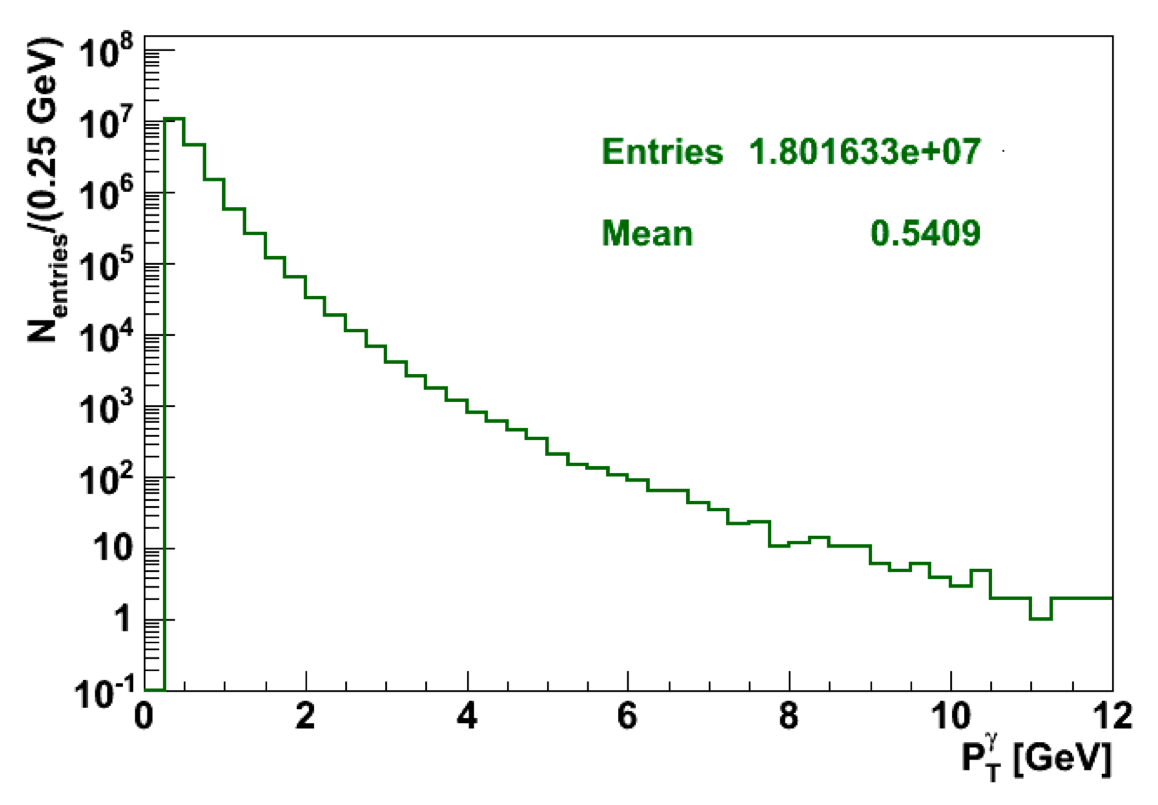
\includegraphics[width=.45\textwidth]{ptMC.png}
\caption{Transverse momentum spectrum of converted photons in minimum
  bias MC events at $\sqrt{s}=900\GeV$.}
\label{ptMC}
\end{figure}

The present analysis makes use of the algorithm described in~\cite{nancy}.
It allows the reconstruction of low-$p_T$ photons ($\geq 0.4\GeV$)
without any request of ECAL match. The main signature for the
conversion identification is the reconstruction of two opposite
charged tracks with tangent direction at the point where they form a
detached vertex. The vertex fit is performed with the \emph{Kinematic
  Constraint Vertex Fitter}.





%\section{Analysed Samples}
\label{sample}

Results shown in this note have been obtained with the release {\tt 3\_3\_6\_patch3} of {\tt CMSSW}.

Data sample corresponds to the dataset\\
{\tt /MinimumBias/BeamCommissioning09-BSCNOBEAMHALO-Dec19thSkim\_336p3\_v1/RAW-RECO}.\\
The list of analyzed runs and lumisections is taken from the table recommended by the Tracker 
DPG\footnote{https://twiki.cern.ch/twiki/bin/viewauth/CMSTKPOGCollisions900GeVDec\#Run\_and\_LumiSection\_selections},
i.e. all runs at $900\GeV$ with detector in stable conditions and magnet fully operational. 
Runs at $\sqrt{s}=2.36\TeV$ are not included.

As far as Monte Carlo simulation is concerned, a sample of $\sim11$M events of minimum bias at $900\GeV$ is used; this sample features a displaced beam spot reproducing the actual beam spot position as observed in collision data. In particular the dataset is:\\
{\tt /MinBias/Summer09-STARTUP3X\_V8K\_900GeV-v1/GEN-SIM-RECO}.

Events are selected with the following requirements:
\begin{itemize}
\item Trigger: bits 0 and 40, plus a veto of beam-halo triggers (bits 36-39); in MC events only bit 40 is required;
\item beam scraping events are rejected requiring a fraction of tracks with \emph{highPurity} quality label greater than 20\%;
\item a {\em good} reconstructed primary vertex is required; a reconstructed primary vertex is defined as good if it originates at least four tracks and if its position lies within $15\cm$ in the longitudinal 
direction and within $2\cm$ in the transverse plane.
\end{itemize}

The results shown in this note are normalized to the number of events surviving the above described selection; in particular 257,526 for data and 6,142,518 for MC, thus the weight applied to MC entries is $4.2\cdot 10^{-2}$. 


%\section{Data and MC Performance}
\label{dataVsMc}
Given the limited number of recorded events passing the trigger and
vertex requirements, the collected statistics allow us to investigate
only the pixel barrel vlolume, that is the tracker region presently
giving the best performance in terms of conversion reconstruction.

A sample of conversions in this region is selected by applying the
following cuts designed to guarantee a good balance between purity and
efficiency:
\begin{itemize}
\item tracks with at least 4 hits;
\item track $d_0\cdot q > 0.1\cm$;
\item track pair opening angle on X-Y plane $\Delta\phi<0.2$;
\item reconstructed conversion vertex radius comprised in the region between $0.8$ and $18\cm$;
\item reconstructed conversion vertex longitudinal position $|z|< 26\cm$;
\item reconstructed transverse momentum of the converted photon $p_T<5\GeV$.
\end{itemize}

Expected performance in terms of efficiency and purity have been
estimated on the MC sample.
Efficiency is defined as the number of associated conversions
$N^{\rm assoc}_{\gamma}$ divided by the total number of simulated
conversions $N^{\rm sim}_{\gamma}$, while purity is defined as
$N^{\rm assoc}_{\gamma}$ divided by the number of reconstructed
conversions $N^{\rm reco}_{\gamma}$.
A reconstructed conversion is considered associated if simulated and reconstructed vertex positions match within a $10\times10\times10\cm^3$ 
box\footnote{A more proper association criteria, based on the hit
  association of the electron tracks, cannot be applied on the used MC
  sample. However, it was proven that the hit and vertex position
  association methods provide compatible results.}.
Figure~\ref{efficpurity} shows that performance degrade for radii greater than $5\cm$, i.e. outside the first pixel barrel layer.
Likely the main reason for this effect is the current tracking configuration where very low $p_T$ tracks can be reconstructed only by using pixel hit triplets as seeds. A different tune of $p_T$ thresholds in iterative tracking steps  could improve performance at larger radii.
%efficiency
%purity
\begin{figure}[!hbtp]
\subfigure[]{
\centering
\label{efficpurity_vs_r}
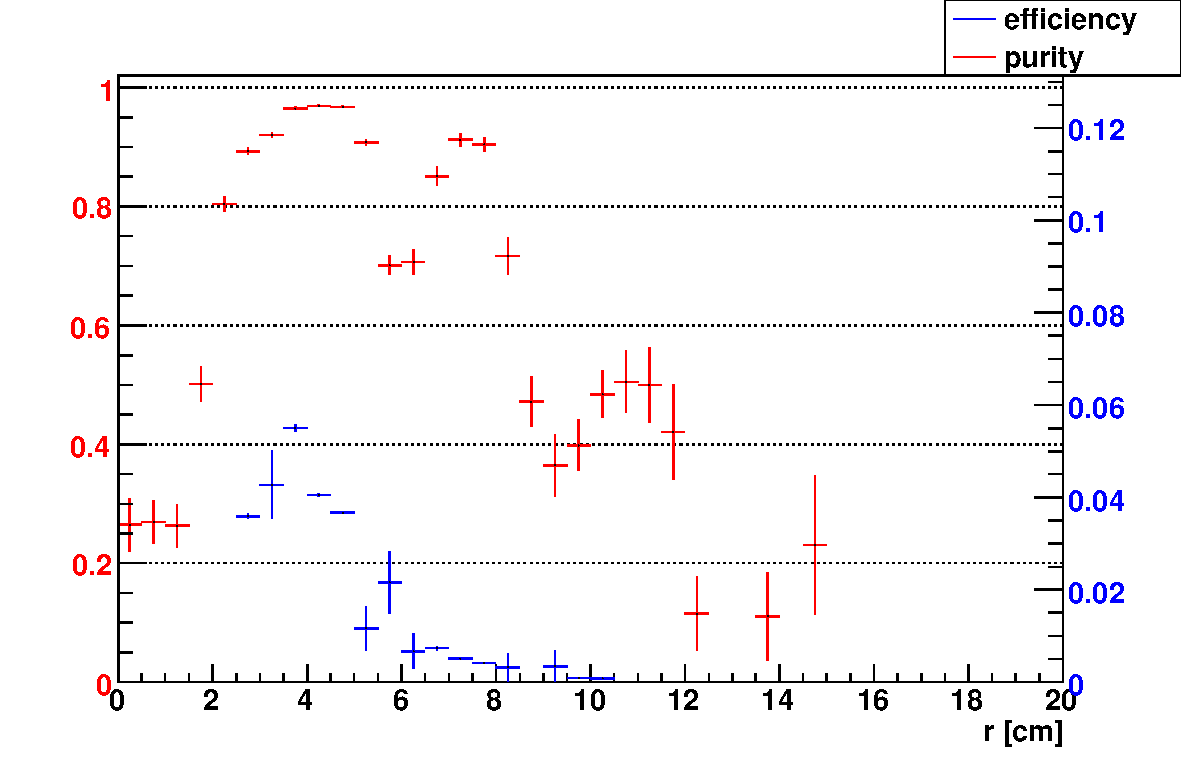
\includegraphics[width=.49\textwidth]{efficpurity_vs_r.pdf}}
\subfigure[]{
\centering
\label{efficpurity_vs_pt}
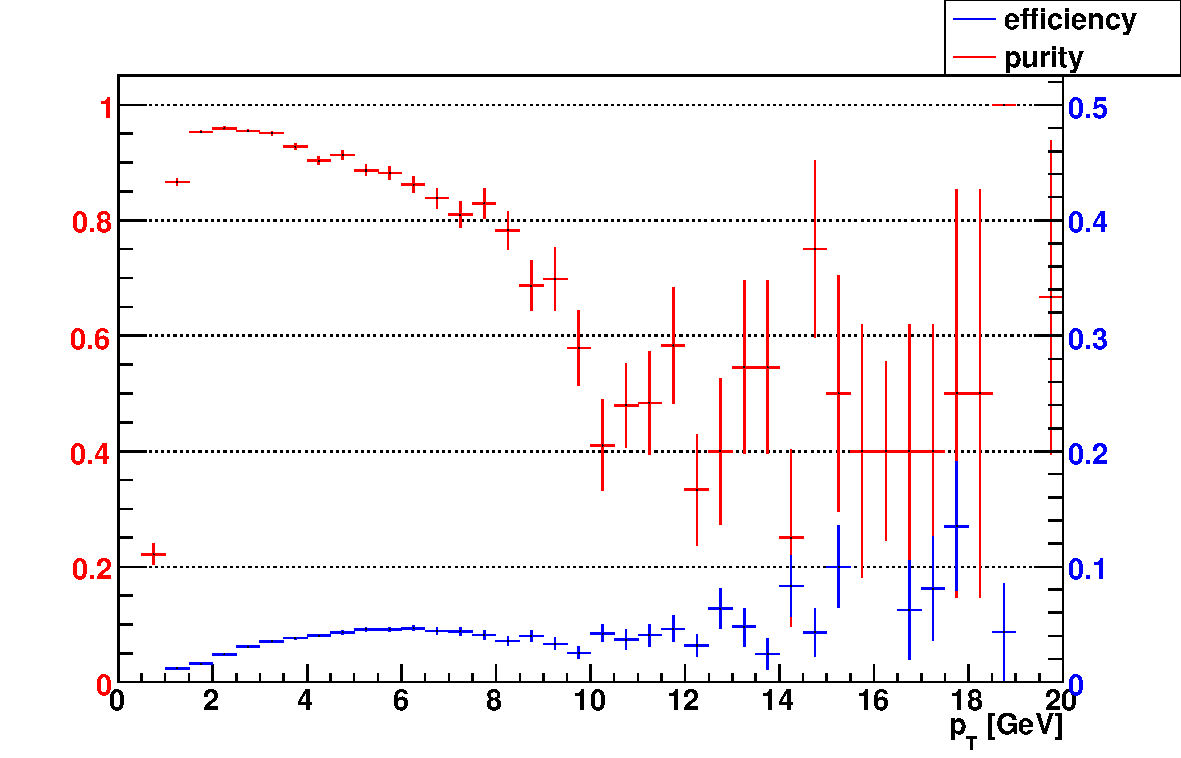
\includegraphics[width=.49\textwidth]{efficpurity_vs_pt.pdf}}
\caption{Efficiency (blue) and purity (red) of the Tracker-only conversion finding algorithm: \subref{efficpurity_vs_r} as a function of $r$; \subref{efficpurity_vs_pt} as a function of $p_T$.}
\label{efficpurity}
\end{figure}

Data versus Monte Carlo simulation comparison has been done on some basic distributions to check the conversion finding algorithm performances with first collision data. The distributions of the reconstructed transverse momentum ($p^{\gamma}_T$) and of the pseudo-rapidity ($\eta^\gamma$) of the converted photon are shown in Fig. ~\ref{fig:pt} and Fig.~\ref{fig:eta}, respectively. The radius of the conversion vertex ($r$) distribution is shown in Fig.~\ref{fig:r}. 

All distributions, given either in linear and in logarithmic scale, result in a pretty good agreement between data and Monte Carlo as far as the shapes are concerned. The overall number of conversions candidates is $\sim10\%$ higher in data with respect to the Monte Carlo simulation. Such small discrepancy is acceptable for the sake of the present preliminary study. It could be due, among several effects, to differences between data and simulation in the number of fakes or at the level of the photon flux.
\begin{figure}[!hbtp]
\centering
\subfigure[]{
\label{subfig:pt_lin}
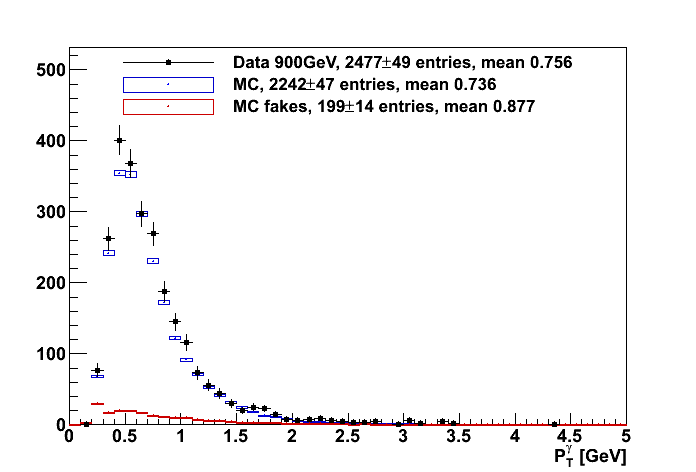
\includegraphics[width=.49\textwidth]{pt_lin.png}}
\subfigure[]{
\label{subfig:pt_log}
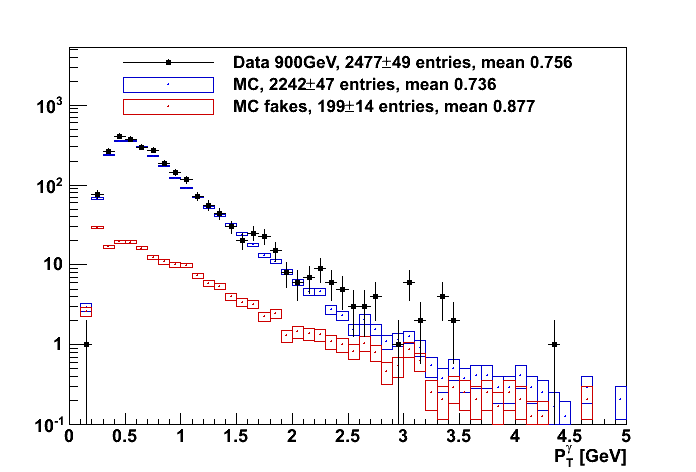
\includegraphics[width=.49\textwidth]{pt_log.png}}
\caption{Distribution of the reconstructed tranverse momentum ($p^{\gamma}_T$) of the converted photon in linear~\subref{subfig:pt_lin} and logarithmic~\subref{subfig:pt_log} scale. Data is shown in black dots and Monte Carlo  simulation in blue boxes. Red boxes represent the estimated fake contribution.}
\label{fig:pt}
\end{figure}

\begin{figure}[!hbtp]
\centering
\subfigure[]{
\label{subfig:eta_lin}
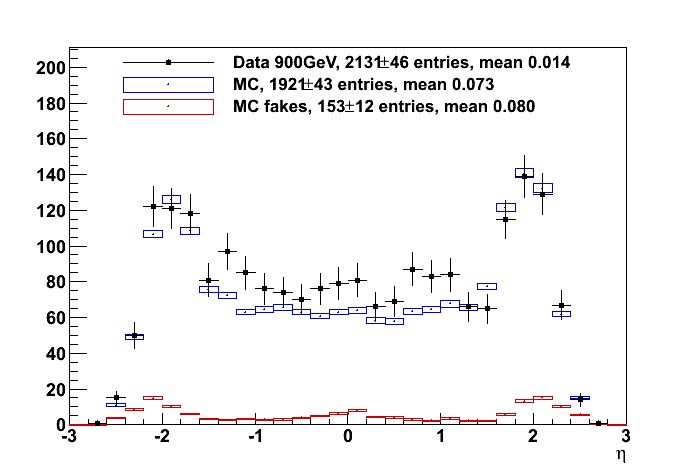
\includegraphics[width=.49\textwidth]{eta_lin.png}}
\subfigure[]{
\label{subfig:eta_log}
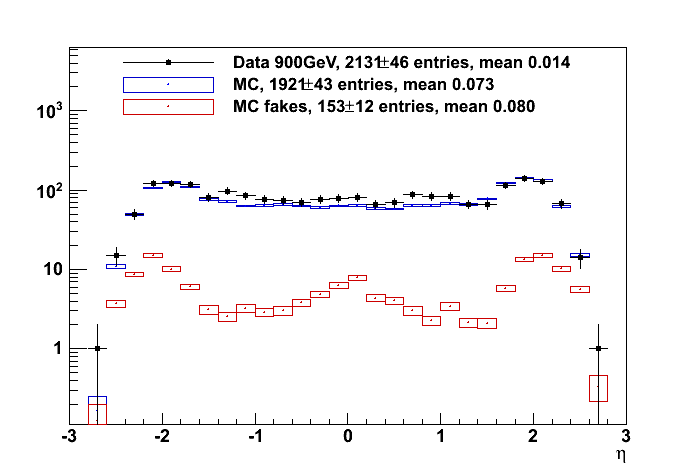
\includegraphics[width=.49\textwidth]{eta_log.png}}
\caption{Distribution of the reconstructed pseudorapidity ($\eta^\gamma$) of the converted photon in linear~\subref{subfig:eta_lin} and logarithmic~\subref{subfig:eta_log} scale. Data is shown in black dots and Monte Carlo  simulation in blue boxes. Red boxes represent the estimated fake contribution.}
\label{fig:eta}
\end{figure}

\begin{figure}[!hbtp]
\centering
\subfigure[]{
\label{subfig:r_lin}
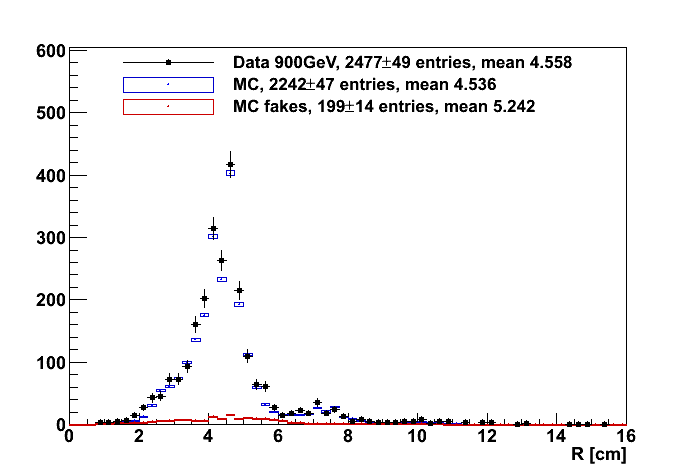
\includegraphics[width=.49\textwidth]{r_lin.png}}
\subfigure[]{
\label{subfig:r_log}
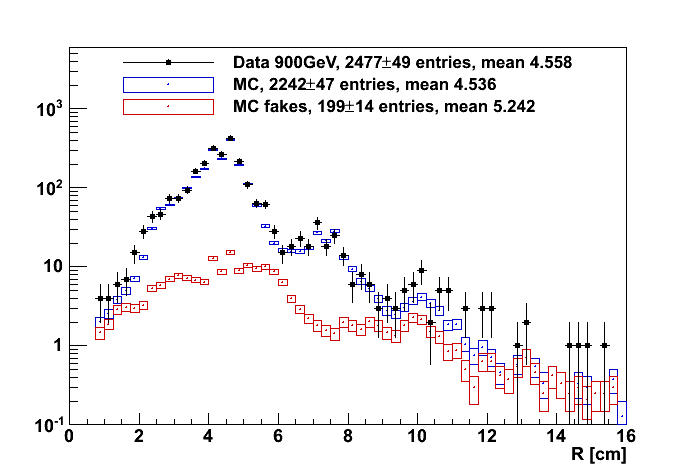
\includegraphics[width=.49\textwidth]{r_log.png}}
\caption{Distribution of the reconstructed conversion radius ($r$) in linear~\subref{subfig:r_lin} and logarithmic~\subref{subfig:r_log} scale. Data is shown in black dots and Monte Carlo simulation in blue boxes. Red boxes represent the estimated fake contribution.}
\label{fig:r}
\end{figure}


%\section{Material Budget Estimation}
\label{correctionFactors}

The following approach to the material budget estimation is along the lines of ref.~\cite{steve}. 

The number of photon conversions $dN_{\rm conv}$ in a
small volume filled with a homogenous material is:
\begin{equation}
dN_{\rm conv} = dN_{\gamma} \frac{P}{X_0} dt .
\label{eq:1}
\end{equation}
where: $dN_\gamma$ is the number of impinging photons; $P$ is the energy dependent conversion probability per unit
radiation length ($P\sim 7/9$); $dt$ is the volume effective thickness (i.e. with respect to the photon arrival direction); $X_0$ is the radiation length (in $\cm$).

Given a portion $R^2 \sin \theta\, d\theta\, d\phi$ centered in $(R,\theta,\phi)$ of a homogenous spherical skin of 
thickness $dR$ in a spherical reference system $(R, \theta, \phi)$,
relation~(\ref{eq:1}) is:
\begin{equation}
dN_{\rm conv} = N_{\gamma}(R, \theta, \phi) \cdot R^2 \sin \theta \, d\theta\, d\phi \cdot \frac{P}{X_0} dR \;,
\label{eq:2}
\end{equation}
where $N_\gamma(R,\theta,\phi)$ is the photon flux impinging the surface element.

However in a particle physics experiment the most common geometrical
structure is a cylindrical skin for which cylindrical reference system
is more appropriate and in some case also cartesian reference system
is convenient.


% \noindent{\bf Pseudo-cylindrical reference system.} 
% In a pseudo-cylindrical
% reference system $(r,\theta,\phi)$ ($r=R\sin\theta$), the relation~(\ref{eq:2}) can be
% conveniently rewritten having care of using the appropriate Jacobian
% factor, i.e.
% \begin{equation}
%  dr\, d\theta\, d\phi = \left| \frac{dr\,d\theta\,d\phi}{dR\,d\theta\,d\phi}
%    \right| \cdot dR\,d\theta\,d\phi
% \label{eq:3}
% \end{equation}
% where
% \begin{equation}
% \begin{split}
% \frac{dr\,d\theta,d\phi}{dR\,d\theta\,d\phi}
% & = \det \left( \begin{array}{ccc}
% \nicefrac{dr}{dR}      & \nicefrac{dr}{d\theta}      & \nicefrac{dr}{d\phi} \\
% \nicefrac{d\theta}{dR} & \nicefrac{d\theta}{d\theta} & \nicefrac{d\theta}{d\phi} \\
% \nicefrac{d\phi}{dR}   & \nicefrac{d\phi}{d\theta}   & \nicefrac{d\phi}{d\phi}
% \end{array} \right) =\\
% & = \det \left( \begin{array}{ccc}
% \sin \theta & R\cos \theta & 0\\
%  0 & 1 & 0 \\
%  0 & 0 & 1 
% \end{array} \right)
% = \sin \theta .
% \end{split}
% \label{eq:4}
% \end{equation}
% Using~(\ref{eq:4}) in~(\ref{eq:2}) we get:
% \begin{equation}
% dN_{\rm conv} = N_{\gamma}(r, \theta, \phi) 
% \frac{P}{X_0} \frac{r^2}{\sin^2\theta} \,dr\,d\theta\,d\phi .
% \label{eq:5}
% \end{equation}

\noindent{\bf Cylindrical reference system.} 
In a cylindrical reference system $(r,z,\phi)$ ($r=R\sin\theta$, $z=R\cos\theta$) the relation~(\ref{eq:2}) can be
conveniently rewritten having care of using the appropriate Jacobian
factor, i.e.
\begin{equation}
 dr\,dz\,d\phi = \left| \frac{dr\, dz\, d\phi}{dR\,d\theta\,d\phi}
   \right| \cdot dR\,d\theta\,d\phi
\label{eq:3bis}
\end{equation}
where
\begin{equation}
\begin{split}
\frac{dr\,dz\,d\phi}{dR\,d\theta\, d\phi}
& = \det \left( \begin{array}{ccc}
\nicefrac{dr}{dR}      & \nicefrac{dr}{d\theta}      & \nicefrac{dr}{d\phi} \\
\nicefrac{dz}{dR}      & \nicefrac{dz}{d\theta}      & \nicefrac{dz}{d\phi} \\
\nicefrac{d\phi}{dR}   & \nicefrac{d\phi}{d\theta}   & \nicefrac{d\phi}{d\phi}
\end{array} \right) = \\
& = \det \left( \begin{array}{ccc}
\sin \theta & R\cos\theta  & 0\\
\cos\theta  & -R\sin\theta & 0 \\
 0 & 0 & 1 
\end{array} \right)
= R .
\end{split}
\label{eq:4bis}
\end{equation}
Using~(\ref{eq:4bis}) in~(\ref{eq:2}) we get:
\begin{equation}
dN_{\rm conv} = N_{\gamma}(r, z, \phi) 
\frac{P}{X_0} r\, \,dr\,dz\,d\phi .
\label{eq:5bis}
\end{equation}

\noindent{\bf Cartesian reference system.} 
Similarly, in a cartesian reference system $(x, y, z)$ ($x=R\sin\theta\cos\phi$, $y=R\sin\theta\sin\phi$, $z=R\cos\theta$)
\begin{equation}
 dx\,dy\,dz  = \left| \frac{dx\, dy\, dz}{dR\,d\theta\,d\phi}
   \right| \cdot dR\,d\theta\,d\phi
\label{eq:3tris}
\end{equation}
where
\begin{equation}
\begin{split}
\frac{dx\,dy\,dz}{dR\,d\theta\,d\phi}
& = \det \left( \begin{array}{ccc}
\nicefrac{dx}{dR}      & \nicefrac{dx}{d\theta}      & \nicefrac{dx}{d\phi} \\
\nicefrac{dy}{dR}      & \nicefrac{dy}{d\theta}      & \nicefrac{dy}{d\phi} \\
\nicefrac{dz}{dR}      & \nicefrac{dz}{d\theta}   & \nicefrac{dz}{d\phi}
\end{array} \right)
= \\
& = \det \left( \begin{array}{ccc}
\sin\theta\cos\phi & R\cos\theta\cos\phi & -R\sin\theta\sin\phi\\
\sin\theta\sin\phi & R\cos\theta\sin\phi &  R\sin\theta\cos\phi\\
\cos\theta & -R\sin\theta & 0 
\end{array} \right)
= \\
& = R^2 \sin \theta = \sqrt{x^2+y^2}\sqrt{x^2+y^2+z^2}.
\end{split}
\label{eq:4tris}
\end{equation}
Using~(\ref{eq:4bis}) in~(\ref{eq:2}) we get:
\begin{equation}
dN_{\rm conv} = N_{\gamma}(x, y, z) 
\frac{P}{X_0}
%\frac{\sqrt{x^2+y^2+z^2}}{\sqrt{x^2+y^2}}
 \,dx\,dy\,dz .
\label{eq:5tris}
\end{equation}

\noindent{\bf Photon flux.} 
A reasonable but approximate guess of the form of
$N_{\gamma}(R, \theta, \phi)$ in the pp collisions at LHC can be
inferred assuming the following:
\begin{itemize}
\item[a)] all photons are originating at the interaction point $(0, 0, 0)$;
\item[b)] all photons come from QCD events ($\pi_0$ decays);
\item[c)] the number of photons interacting with the material is negligible. 
\end{itemize}
All these three assumption are to some extent not true, c) especially,
but let's give them for granted for the present preliminary study.

%\clearpage

The dependence on the distance from the interaction point is easily inferred observing that, givem the above assumptions, 
the flux is the same in the same portion of solid angle $\delta \Omega=\sin \theta\delta\theta d\phi$:%$\d \Omega=\sin \theta\d\theta d\phi$: 
\begin{equation}
N_{\gamma}(R', \theta, \phi) R'^2 d\Omega = N_{\gamma}(R, \theta, \phi) R^2 d\Omega,
\label{eq:6pre}
\end{equation}
from which immediately follows that
\begin{equation}
N_{\gamma}(R) \propto \frac{1}{R^2} = \frac{\sin^2 \theta}{r^2} = \frac{1}{x^2+y^2+z^2} .
\label{eq:6}
\end{equation}

As a consequence of the cylindrical symmetry of pp interactions
$N_\gamma$ does not depend on $\phi$.

%As far as the $\theta$ dependance is concerned
Given the definition of pseudorapidity, 
\begin{equation}
\eta = -\ln \left( \tan \nicefrac{\theta}{2} \right)
\label{eq:7}
\end{equation}
it follows that the differential in $\eta$ is related to the differential in $\cos\theta$:
% \begin{equation}
% \begin{split}
% dN_\gamma & = N_\gamma(\eta) d\eta  =
% N_\gamma(\eta)\frac{d\eta}{d\cos\theta} d\cos\theta = N_\gamma(\eta)\frac{d\eta}{d\theta}\frac{d\theta}{d\cos\theta} d\cos\theta=\\ 
%  & =N_\gamma(\eta)\frac{1+\tan^2\nicefrac[]{\theta}{2}
%  }{2\tan\nicefrac{\theta}{2}} \frac{1}{\sin\theta} d\cos\theta =
%  N_\gamma(\eta)\frac{1}{2\sin\nicefrac[]{\theta}{2}\cos\nicefrac[]{\theta}{2}} \frac{1}{\sin\theta}  d\cos\theta  
%  = N_\gamma(\eta)\frac{1}{\sin^2\theta}  d\cos\theta .
% \label{eq:8}
% \end{split}
% \end{equation}
\begin{equation}
\begin{split}
d\eta  = &
\frac{d\eta}{d\cos\theta} d\cos\theta = \frac{d\eta}{d\theta}\frac{d\theta}{d\cos\theta} d\cos\theta=\\ 
 & =\frac{1+\tan^2\nicefrac[]{\theta}{2}
 }{2\tan\nicefrac{\theta}{2}} \frac{1}{\sin\theta} d\cos\theta =
 \frac{1}{2\sin\nicefrac[]{\theta}{2}\cos\nicefrac[]{\theta}{2}} \frac{1}{\sin\theta}  d\cos\theta  
 = \frac{1}{\sin^2\theta}  d\cos\theta .
\label{eq:8pre}
\end{split}
\end{equation}
Since 'all' photons come from $\pi_0$'s that show a flat
distribution as the function of rapidity that here is confused with $\eta$, also photon $\eta$-distribution is flat.
This fact can be used, together with relation~(\ref{eq:8pre}), can be used as follows:
\begin{equation}
\begin{split}
{\rm cost}\cdot\left( \eta_2 - \eta_1 \right)\cdot\left( \phi_2 - \phi_1 \right) = & \int_{\eta_1}^{\eta_2}\int_{\phi_1}^{\phi_2} {\rm cost}\cdot d\eta\, d\phi = \int_{\eta_1}^{\eta_2}\int_{\phi_1}^{\phi_2} {\rm cost}\cdot \frac{d\cos \theta}{\sin^2 \theta} d\phi = \\
= & \int_{\theta(\eta_1)}^{\theta(\eta_2)}\int_{\phi_1}^{\phi_2} N_\gamma(\theta)\cdot d\cos \theta\, d\phi .
\label{eq:8}
\end{split}
\end{equation}
Relation~(\ref{eq:8}) allows to identify $N_\gamma(\theta)$ with ${\rm cost}/\sin^2{\theta}$ so that
\begin{equation}
N_\gamma(\theta) \propto \frac{1}{\sin^2 \theta} = \frac{x^2+y^2+z^2}{x^2+y^2}.
\label{eq:9}
\end{equation}
Putting~(\ref{eq:6}) and~(\ref{eq:9}) together we get 
\begin{equation}
N_{\gamma} (R, \theta, \phi) = k \frac{1}{R^2\sin^2 \theta} \, \, \, ,
\label{eq:10pre}
\end{equation}
% \begin{equation}
% N_{\gamma} (r, \theta, \phi) = k \frac{\sin \theta}{r^2} \,\,\, ,
% \label{eq:10}
% \end{equation}
\begin{equation}
N_{\gamma} (r, z, \phi) = k \frac{1}{r^2} \,\,\, ,
\label{eq:10bis}
\end{equation}
and
\begin{equation}
N_{\gamma} (x, y, z) = k \frac{1}{x^2+y^2} \,\,\, ,
\label{eq:10tris}
\end{equation}
for spherical,
%pseudo-cylindrical, 
cylindrical and cartesian coordinates
respectively. In all cases $k$ is an appropriate dimensional factor
that accounts for all necessary constants.

\noindent{\bf Geometrical dependence of photon conversions.} 
Equations
%~(\ref{eq:5}) with~(\ref{eq:10}),
~(\ref{eq:5bis})
with~(\ref{eq:10bis}), and~(\ref{eq:5tris}) with~(\ref{eq:10tris}),
respectively, allow for the following expressions for the number of photon
conversion to be written:
\begin{equation}
d N_{\rm conv} = k \frac{1}{r^2} 
\frac{P}{X_0} r dr\, dz\, d\phi = k
\frac{P}{X_0} \frac{1}{r}\, dr\, dz\, d\phi ,
\label{eq:11bis}
\end{equation}
\begin{equation}
\begin{split}
d N_{\rm conv} & = k \frac{P}{X_0} \frac{1}{x^2+y^2} \,dx\,dy\,dz .
\end{split}
\label{eq:11tris}
\end{equation}
After the appropriate integration,
%Eq.~(\ref{eq:11}),
Eq.~(\ref{eq:11bis}) and~(\ref{eq:11tris}) can be used to extract the
geometrical factor to translate the observed number of conversion in a given 
volume into an estimate of $P/X_0$ (for the moment let's assume that
the conversion reconstruction efficiency is 1 with no background).

Few relevant examples follow.

\begin{description}
% \item[$r_1<r<r_2$,~$\, \theta_1<\theta<\theta_2$,~$\, 0<\phi<2\pi$;]
%   from~Eq.~(\ref{eq:11}): 
% \begin{equation}
% \begin{split}
% N_{\rm conv} & = k \frac{P}{X_0} \int_{\theta_1}^{\theta_2}
% \frac{d\theta}{\sin\theta} \int_{r_1}^{r_2}dr \int_0^{2\pi}d\phi = \\
% & = 2\pi k \frac{P}{X_0} (r_2-r_1) \cdot \left. \ln \tan
%     \frac{\theta}{2} \right|_{\theta_1}^{\theta_2} =\\
% & = 2\pi k \frac{P}{X_0} (r_2-r_1) (\eta_1 - \eta_2).
% \end{split}
% \label{eq:12}
% \end{equation}
%
%%%%% Versione precendete (ma da conservare perche` forse e` il conteggio dei fotoni)
%
\item[$r_1<r<r_2$,~$\, z_1<z<z_2$,~$\, 0<\phi<2\pi$;]
  from~Eq.~(\ref{eq:11bis}): 
\begin{equation}
\begin{split}
N_{\rm conv} & = k
\frac{P}{X_0} \int_{r_1}^{r_2} \frac{dr}{r} \int_{z_1}^{z_2} dz
\int_0^{2\pi} d\phi = \\
& = 2\pi k \frac{P}{X_0}  (z_2 - z_1) \ln \frac{r_2}{r_1} \equiv k \frac{P}{X_0} f^{r, z}_{\rm geom}.\\
\end{split}
\label{eq:13}
\end{equation}
%
%%%%%%%%%%%%%%%%%%%%%%%%%%%%%%%%%%%%%%%%%%%%%%%%%%%%
%%%%% Versione precendete (ma da conservare perche` forse e` il conteggio dei fotoni)
%
% \item[$r_1<r<r_2$,~$\, z_1<z<z_2$,~$\, 0<\phi<2\pi$;]
%   from~Eq.~(\ref{eq:11bis}): 
% \begin{equation}
% \begin{split}
% N_{\rm conv} & = k
% \frac{P}{X_0} \int_{r_1}^{r_2} \int_{z_1}^{z_2} \frac{dr \, dz}{\sqrt{r^2+z^2}}
% \int_0^{2\pi} d\phi = \\
% & = 2\pi k \frac{P}{X_0} \int_{r_1}^{r_2} dr \left. \ln \left( 2\sqrt{r^2+z^2}+2z \right) \right|_{z_1}^{z_2} = \\
% & = 2\pi k \frac{P}{X_0} \int_{r_1}^{r_2} dr \ln \frac{\sqrt{r^2+{z_2}^2}+z_2}{\sqrt{r^2+{z_1}^2}+{z_1}} = \\ 
% & = 2\pi k \frac{P}{X_0} \left[ r \ln \frac{\sqrt{r^2+{z_2}^2}+z_2}{\sqrt{r^2+{z_1}^2}+{z_1}} + \right. \\
% & - z_1 \ln \left( 2\sqrt{r^2+{z_1}^2}+r \right)  + \Biggl. \Biggl. z_2 \ln \left( 2\sqrt{r^2+{z_2}^2}+r \right) \Biggr] \Biggr|_{r_1}^{r_2} = \\
% & = 2\pi k \frac{P}{X_0} \left[ r_2 \ln \frac{\sqrt{{r_2}^2+{z_2}^2}+z_2}{\sqrt{{r_2}^2+{z_1}^2}+z_1} - r_1 \ln \frac{\sqrt{{r_1}^2+{z_2}^2}+z_2}{\sqrt{{r_1}^2+{z_1}^2}+z_1} + \right. \\
% & \left. + z_2 \ln \frac{\sqrt{{r_2}^2+{z_2}^2}+r_2}{\sqrt{{r_1}^2+{z_2}^2}+r_1} - z_1 \ln \frac{\sqrt{{r_2}^2+{z_1}^2}+r_2}{\sqrt{{r_1}^2+{z_1}^2}+r_1} \right] \\
% & \equiv k \frac{P}{X_0} f^{r, z}_{\rm geom}.\\
% \end{split}
% \label{eq:13}
% \end{equation}
%
%%%%%%%%%%%%%%%%%%%%%%%%%%%%%%%%%%%%%%%%%%%%%%%%%%%%
%
\item[$x_1<x<x_2$,~$\, y_1<y<y_2$,~$\, z_1<z<z_2$;]
  from~Eq.~(\ref{eq:11tris}): 
\begin{equation}
\begin{split}
N_{\rm conv} & = k
\frac{P}{X_0} \int_{x_1}^{x_2} \int_{y_1}^{y_2} \frac{dx\,
  dy }{x^2+y^2} \int_{z_1}^{z_2} dz  . 
\end{split}
\label{eq:14}
\end{equation}
The analytical solution~\cite{integrals} of the integral would require the computation of polylogarithmic functions. Within
our needs (i.e. for a scatter plot in the $xy$ plane), if $r\gg |x_2-x_1|$ and $r\gg |y_2
- y_1|$, a likely sufficient approximate
solution is
\begin{equation}
N_{\rm conv} = k
\frac{P}{X_0} \frac{\Delta x\, \Delta y\, \Delta z}{\overline{r}^2} \equiv k \frac{P}{X_0} f^{x, y}_{\rm geom}
\label{eq:15}
\end{equation}
where $\overline{r}$ is the ``average'' transverse radius, i.e. the one taken on
the middle of the ``box'':
\begin{equation}
 \overline{r}=\nicefrac{1}{2}\sqrt{(x_1+x_2)^2+(y_1+y_2)^2}.
\label{eq:16}
\end{equation}
%$\overline{r}=\sqrt{\nicefrac{(x_1+x_2)^2}{4}+\nicefrac{(y_1+y_2)^2}{4}}$.
% \item[$x_1<x<x_2$,~$\, y_1<y<y_2$,~$\, z_1<z<z_2$;]
%   from~Eq.~(\ref{eq:11tris}): 
% \begin{equation}
% \begin{split}
% N_{\rm conv} & = k
% \frac{P}{X_0} \int_{x_1}^{x_2} \int_{y_1}^{y_2} \int_{z_1}^{z_2}  \frac{dx\,
%   dy \, dz}{\sqrt{x^2+y^2}\sqrt{x^2+y^2+z^2}}. 
% \end{split}
% \label{eq:14}
% \end{equation}
% The analytical solution of the integral does not exist~\cite{integrals}. Within
% our needs (i.e. for a scatter plot in the $xy$ plane) we can integrate first in $dz$:
% \begin{equation}
% \begin{split}
% N_{\rm conv} & = k
% \frac{P}{X_0} \int_{x_1}^{x_2} \int_{y_1}^{y_2} dx \, dy \left. \frac{1}{r} \ln \left( 2\sqrt{r^2+z^2} + 2z \right) \right|_{z_1}^{z_2} \\
% & = k \frac{P}{X_0} \int_{x_1}^{x_2} \int_{y_1}^{y_2} dx \, dy  \frac{1}{r} \ln \frac{\sqrt{r^2+{z_2}^2} + z_2}{\sqrt{r^2+{z_1}^2} + z_1} ,
% \end{split}
% \label{eq:15pre}
% \end{equation}
% where $r=\sqrt{x^2+y^2}$. If $r\gg |x_2-x_1|$ and $r\gg |y_2
% - y_1|$, a likely sufficient approximate
% solution is
% \begin{equation}
% \begin{split}
% N_{\rm conv} & = k
% \frac{P}{X_0} \frac{\Delta x\, \Delta y}{\overline{r}} \,  \ln \frac{\sqrt{\overline{r}^2+{z_2}^2} + z_2}{\sqrt{\overline{r}^2+{z_1}^2} + z_1} \\
% & \equiv k \frac{P}{X_0} f^{x, y}_{\rm geom}
% \end{split}
% \label{eq:15}
% \end{equation}
% where $\overline{r}$ is the ``average'' radius, i.e. the one taken on
% the middle of the ``box'', $\overline{r}=\nicefrac{1}{2}\sqrt{(x_1+x_2)^2+(y_1+y_2)^2}$.
% %$\overline{r}=\sqrt{\nicefrac{(x_1+x_2)^2}{4}+\nicefrac{(y_1+y_2)^2}{4}}$.
\end{description}

%\end{document}










  

%\section{Results}
\label{results}

The conversion counting in a given volume can be translated into a material budget estimate once the efficiency and the impinging 
photon flux are correctly taken into account. 
In particular, assuming a negligible background, the number of reconstructed photon conversion $N_{\rm reco}$ in a given volume bin is
\begin{equation}
N_{\rm reco} \propto \varepsilon \cdot \langle \frac{P}{X_0} \rangle \cdot f_{\rm geom}
\end{equation}
where $\varepsilon$ is the reconstruction efficiency and $\langle P/{X_0} \rangle$ is the average conversion probability ($P\sim 7/9$).

The present statistics allow only the pixel barrel to be studied. 
It is identified by choosing the following fiducial volume: $|z|<26~{\rm cm}$ and $r<15~{\rm cm}$.
Such region is divided for convenience in four parts, corresponding to the beam pipe and the three pixel barrel layers:\\
$1~{\rm cm}<r_{\rm BP}<3.5~{\rm cm}<r_{\rm PXL1}<6~{\rm cm}<r_{\rm PXL2}<8.4~{\rm cm}<r_{\rm PXL3}<15~{\rm cm}$. \\
The conversion finding efficiency $\varepsilon$, estimated from MC data for each sub-region, is 2.8\%, 3.5\%, 0.5\% and 0.1\% respectively.

Fig.~\ref{figMBvsr} represents an uncalibrated estimation, given in arbitrary units, 
comparing the material budget of the beam pipe and of the pixel barrel layers as a function of the radius $r$.
The correction factor $f^{r, z}_{\rm geom}$ is given by Eq.~\ref{eq:13}.
The green line shows the case of ideal resolution and efficiency, corrected for $f_{\rm geom}$.
Blue boxes represent MC pseudo data and black dots data; they are both corrected for $\varepsilon$ and $f_{\rm geom}$.
The conversion radius in data is computed with respect to the pixel center $(-0.1475\cm, -0.3782\cm, -0.4847\cm)$, 
as estimated from tracker alignment algorithms. 
The expected fake contribution, shown in red boxes, is not subtracted. 
Data show a good agreement with MC, both in shapes and in the overall number of entries.
The third pixel layer bin is dominated by statistical fluctuations and the high background contribution.

\begin{figure}[!htbp]
 \begin{center}
   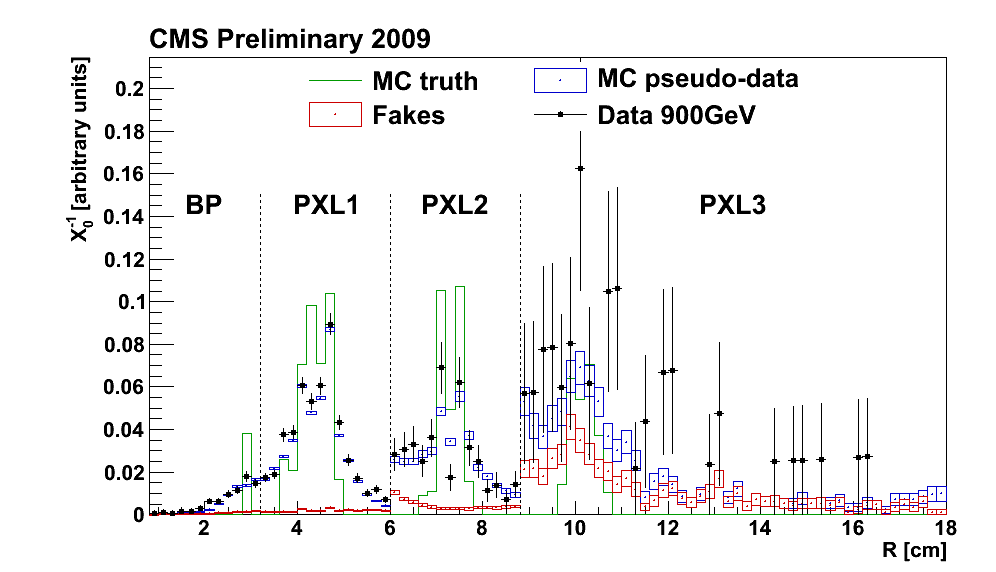
\includegraphics[width=\textwidth]{rPlot.png}
 \end{center}
 \caption{Uncalibrated material budget vs. radius.}
\label{figMBvsr}
\end{figure}

Fig.~\ref{xyPlot} and Fig.~\ref{zrPlot} show the comparison in the $x$$-$$y$ and $z$$-$$r$ planes respectively, where the grey density 
gives an estimate of the amount of material in bins of size $0.25~cm\times0.25~cm$. 
The material in the $x$$-$$y$ plane is computed using the correction factor $f^{x, y}_{\rm geom}$ defined in Eq.~\ref{eq:15}.
The low statistics of reconstructed photon conversions does not allow a quantitative comparison of the results from data yet.

\begin{figure}[!hbtp]
\centering
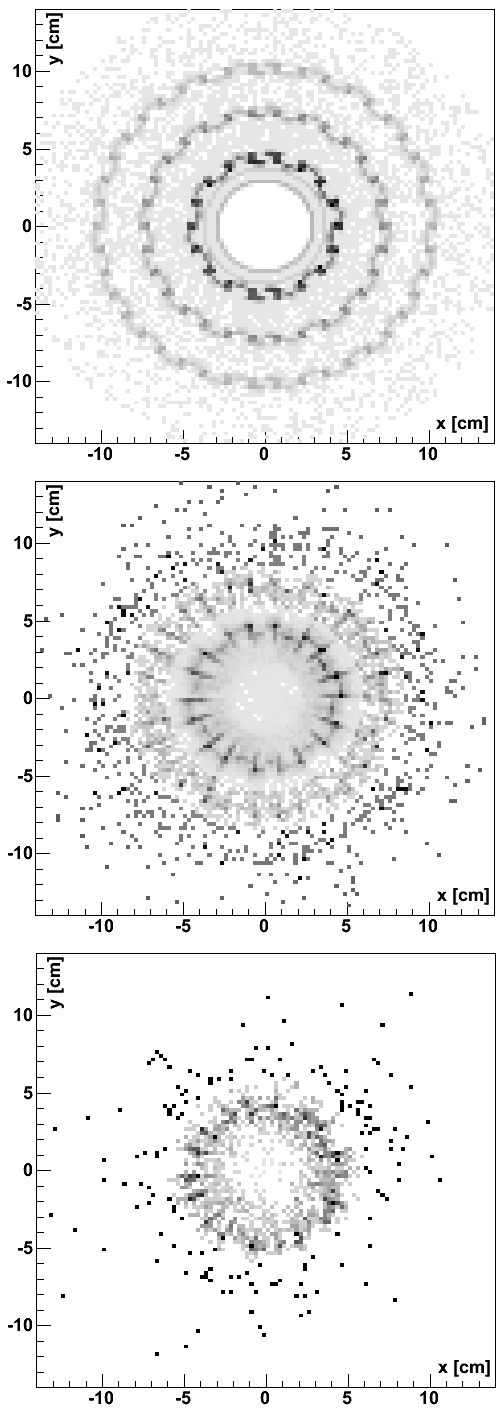
\includegraphics[height=0.9\textheight]{xyPlotVert.png}
\caption{Material budget estimation $x$$-$$y$ map. Top: MC truth; Center: MC pseudo-data; Bottom: data.}
\label{xyPlot}
\end{figure}

\begin{figure}[!hbtp]
\centering
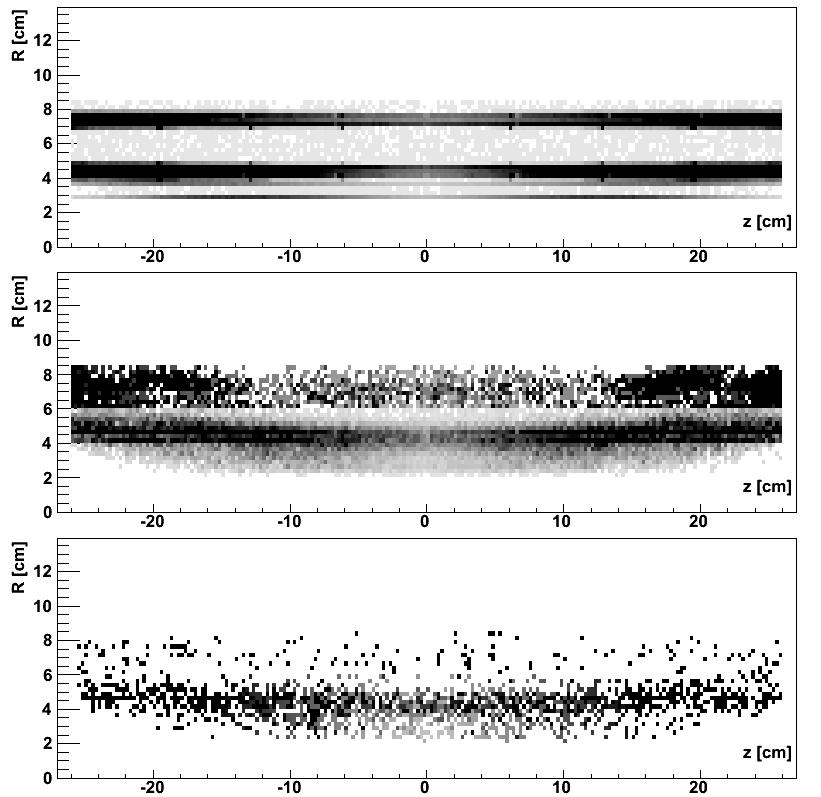
\includegraphics[width=\textwidth]{zrPlot.png}
\caption{Material budget estimation $z$$-$$r$ map. Top: MC truth; Center: MC pseudo-data; Bottom: data.}
\label{zrPlot}
\end{figure}


%\section{Unfolding}
\label{unfolding}

A more complete analysis of the material budget estimate needs to take into account the non ideal conversion vertex position resolution.
In fact, the radius of simulated conversion vertices in the pixel barrel region is well separated in the four peaks due to the beam pipe
and the the pixel layers (Fig.~\ref{Rmc}).


\begin{figure}[|htbp]
 \begin{center}
   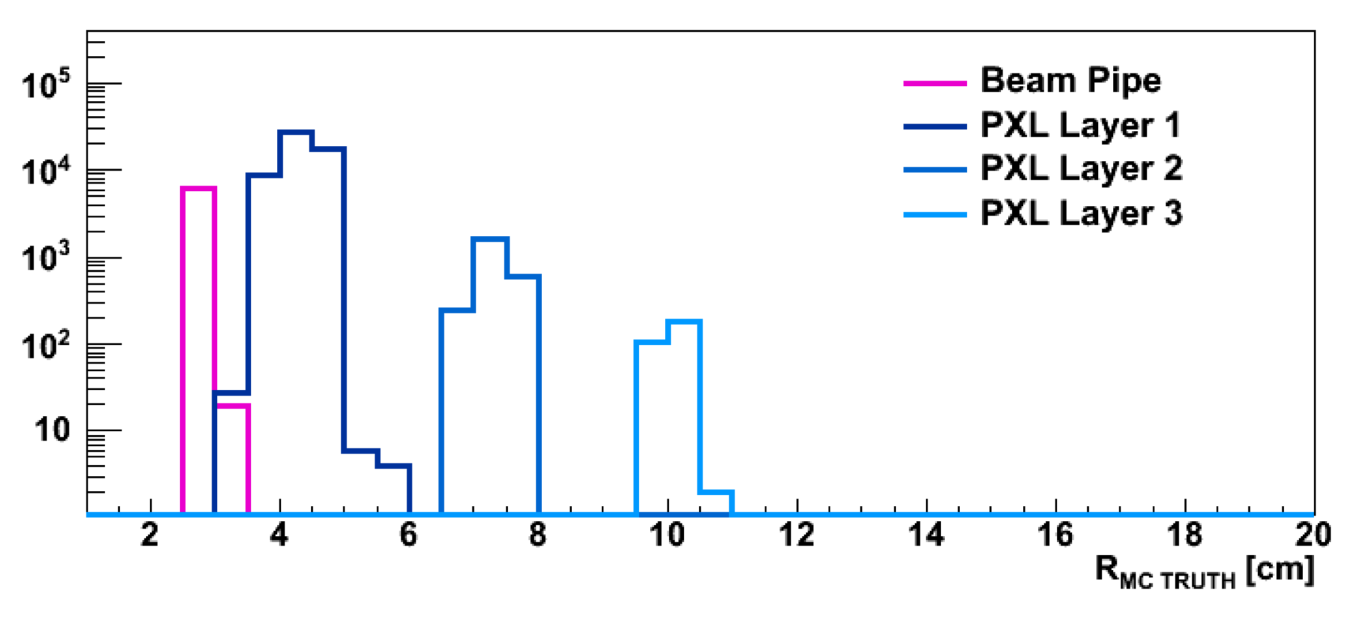
\includegraphics[width=\textwidth]{Rmc.png}
 \end{center}
 \caption{.}
\label{Rmc}
\end{figure}

\begin{figure}[|htbp]
 \begin{center}
   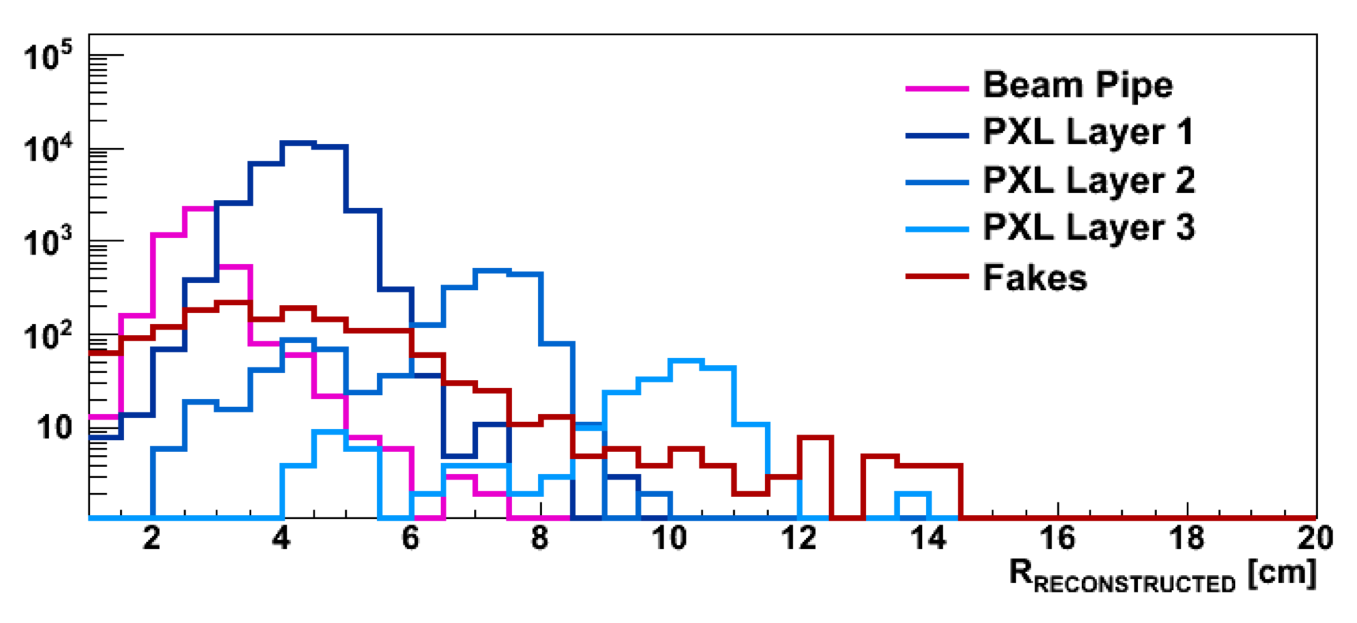
\includegraphics[width=\textwidth]{Rreco.png}
 \end{center}
 \caption{.}
\label{Rreco}
\end{figure}


%%\thispagestyle{empty}
\section{Conclusions}
\label{conclusions}


%%\newpage
\section*{References}

\begin{thebibliography}{99}
\bibitem{cms}
  Adolphi R et al. [CMS Collaboration] 2008 The CMS experiment at the CERN LHC
  {\em JINST} {\bf 3} S08004 
\bibitem{TkTDR} CMS Collaboration 1998 The Tracker System Project Technical Design Report
  {\em CERN-LHCC} 98-6
\bibitem{TkTDRadd} CMS Collaboration 2000 Addendum to the CMS Tracker TDR {\em
   CERN-LHCC} 2000-16
\bibitem{trackreco} CMS Collaboration 2010 Tracking and Vertexing Results from First Collisions
{\em CMS-PAS} TRK-10-001
\bibitem{cmssw} CMS Collaboration 2006 CMS Physics Technical Design
    Report Detector Performance and Software {\em
      CERN-LHCC} 2006-001
\bibitem{posterConv} Giordano D and Sguazzoni G [CMS
  Collaboration] 2012 An innovative seeding technique for photon conversion
  reconstruction at CMS {\em these proceedings}
\bibitem{kdtree} Bentley J L 1975 Multidimensional binary search
    trees used for associative searching {\em Commun. ACM} {\bf 18} 9 (Sep. 1975) 509-517 
\bibitem{parallel} Hauth T, Innocente V and Piparo D [CMS
  Collaboration] 2012 Development and Evaluation of Vectorised and
    Multi-Core Event Reconstruction Algorithms within the CMS Software
    Framework {\em these proceedings}
\end{thebibliography}


\end{document}
